\chapter[Introduction]{Introduction}

\section{Background}

Due to the increased popularity of online classes and the rising enrollment in foundational science and \index{engineering}engineering courses, professors and teaching assistants are under constant pressure to provide students with the assistance that they need throughout the semester - especially on homework assignments. When direct help from a faculty member is not available, students need an interactive learning tool that guides them through homework problems. This is especially important in an environment where nontraditional students with diverse schedules must attend class\cite{choy2002, horn1996}. Student success in any course requires good communication between students and instructors. However, the expectation of access to faculty at any time is unrealistic with all of the duties of the teaching staff.

We are developing a \gls{cita} for the calculus-based introductory electricity and magnetism course for engineers at Purdue University. This program will guide students through homework problems while teaching the nuanced techniques of physics problem solving. The most often heard statement from students attempting a physics problem is, ``I don’t even know where to begin.'' Our goal is to design an interactive component for every homework problem that will develop help students generate an understanding of physics concepts and enchance their problem solving skills.

Most computerized homework systems only provide a ``correct'' or ``incorrect'' response to an answer. If a student receives the ``incorrect'' message, there is no explanation as to why their logic was wrong. Even worse, these systems do not provide instruction on how to proceed from the point at which the student made a mistake. Sometimes, there is a link to a passage in the textbook that lists the derivation of the problem without specific context. At this point, the student either has to email an instructor, wait for recitation later in the week, or seek special appointments with instructors. Thus, the learning process is interrupted as the student waits for simple guidance. Our goal is to design, develop, implement, and analyze an online system that is available at any time to provide focused guidance to help students acquire the knowledge and skills necessary to solve the problem.

% !! Seek help from classmates with similar difficulties !!
% Benefit of the system - it's ok if students have similar difficulties. Knowledge becomes more public
% -> Add Lit review from wendy wampler's thesis
% -> Add Polya's book, it's foundational...
% -> Add Mazur's book

\section{Overview of Electricity and Optics at Purdue}

This study takes place in.... ...which
Italicize textbook titles

PHYS 24100 and PHYS 24100D (Electricity and Optics) are the introductory electromagnetism courses for \index{engineering}engineering majors at Purdue University. The ``D'' represents that it is a distance learning course (i.e. an online course). The content in these two classes is exactly the same; they only differ in the fact that the distance learning sections watch video lectures and attend live online recitations through Cisco WebEx while the regular sections watch live lectures and attend live recitations on campus.

Electricity and Optics is generally taken after students complete PHYS 17200 - Modern Mechanics. This introductory mechanics course is currently taught using the Matter and Interactions textbook by Dr. Ruth Chabay and Dr. Bruce Sherwood\cite{chabay2010}. PHYS 24100 or PHYS 24100D is a prerequisite for many of the intermediate \index{engineering}engineering courses at Purdue University.

Engineering students usually take this course in the fall semester (the ``on-semester''). Alternatively, some students choose to take the course in the spring or summer due to the fact that they are either ahead or behind in their schedules (the ``off-semesters''). Figure \ref{fig:enrollment} shows the total enrollment in PHYS 24100 and PHYS 24100D over the last three years. Note that PHYS 24100D was not created until summer 2012.

Figure \ref{fig:percent} shows the percent of the total class that is enrolled in the distance learning section of Electricity and Optics. It is important to note that although we try to separate the online and on-campus sections, the placement is dependent on student preference. For example, during the summer semester in 2015, we had such a high demand for online courses that we decided to combine all of the sections into PHYS 24100 rather than separating them into PHYS 24100 and PHYS 24100D. Data is not shown in figure \ref{fig:percent} for the year 2015 since it is as of yet incomplete.

\begin{figure}[!hb]
	\centering
	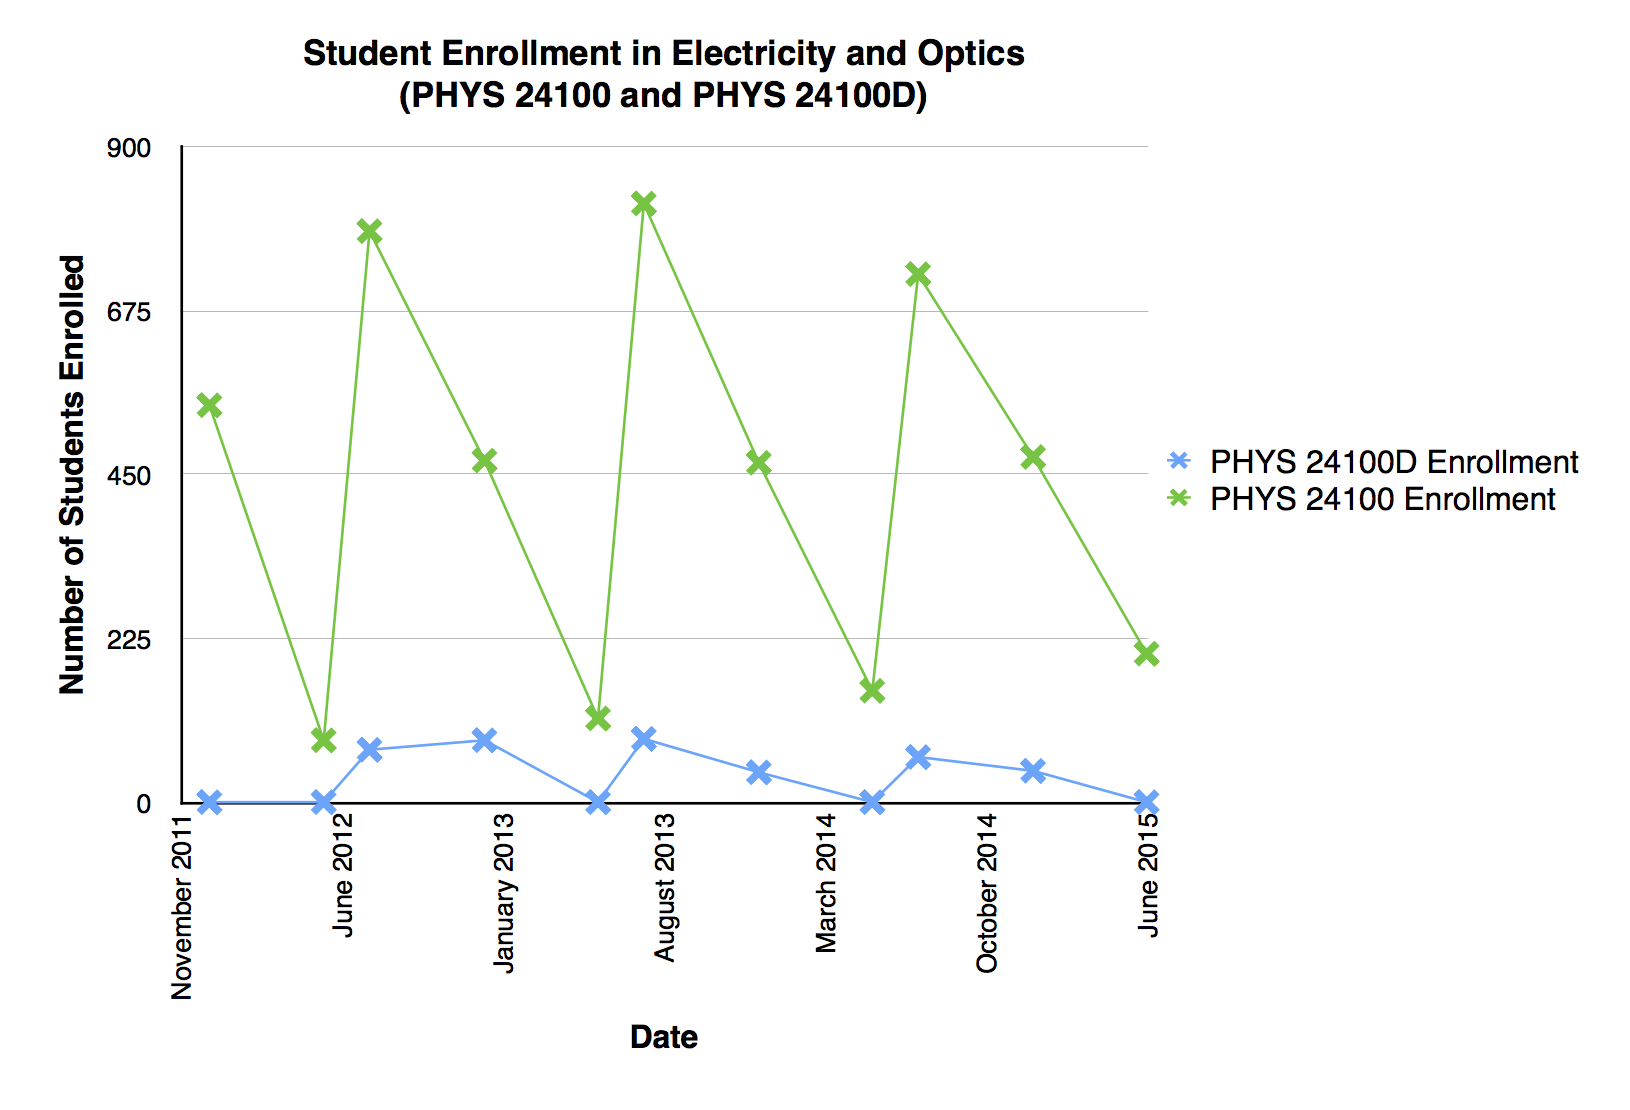
\includegraphics[width=5in]{img/chapter1/enrollment}
	\caption[Enrollment in PHYS 24100 and PHYS 24100D Over the Last Three Years]{Enrollment in PHYS 24100 and PHYS 24100D Over the Last Three Years}
	\label{fig:enrollment}
\end{figure}

% ^Redo this chart^

\begin{figure}[!hb]
	\centering
	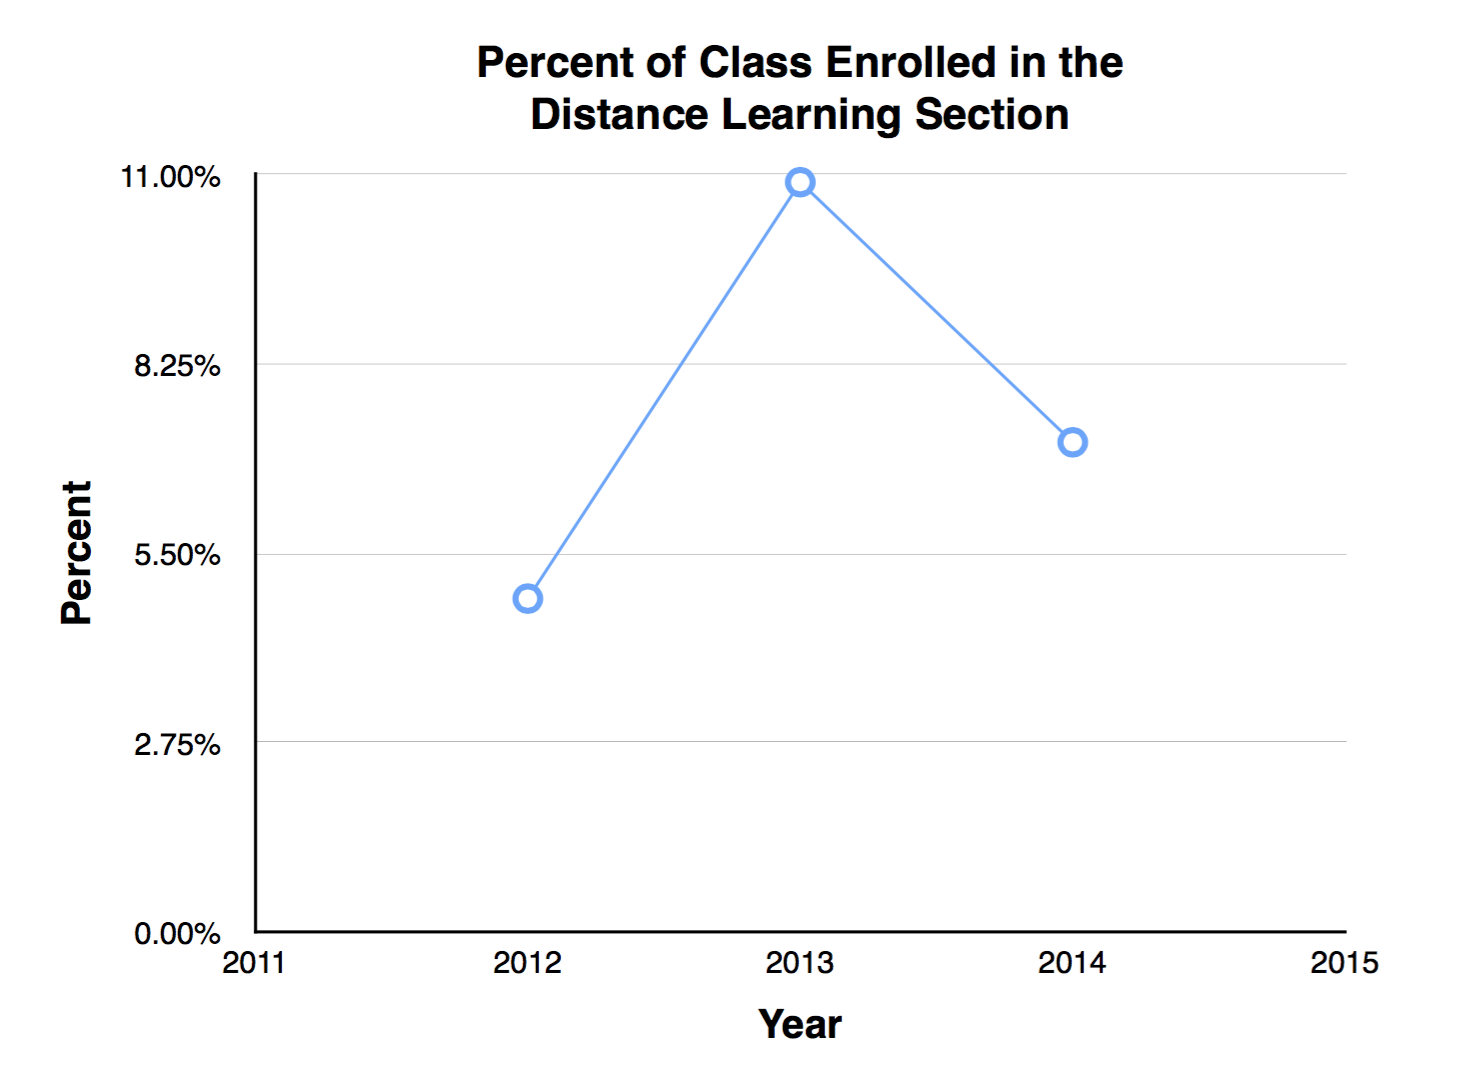
\includegraphics[width=5in]{img/chapter1/percent}
	\caption[Percent of Students in PHYS 24100D (Distance Learning)]{Percent of Students in PHYS 24100D (Distance Learning)}
	\label{fig:percent}
\end{figure}

\section{Overview of Homework in Electricity and Optics}

PHYS 24100 and PHYS 24100D use an in-house homework system called \gls{chip}. The \gls{chip} system is based on the CPlite homework system from the \gls{uiuc}. Purdue University adopted an early version of CPlite in 1997 and continued to make improvements to it over the next decade, adding statistical analysis tools, gradebooks, and updated homework problems. \gls{chip} services not only the introductory electromagnetism courses, but also many of the other physics courses at Purdue University.

% -> Add a couple of references to the CPLite system.

\subsection*{Strengths}

\gls{chip} is a well established system that has over a decade of in-the-field use. One of its biggest advantages is that it has no ties to any external companies or organizations. Faculty members at Purdue are free to recommend updates or modify the source code as they wish. (Rephrase this)

All of the \gls{chip} servers are maintained on Purdue University campus in the physics building by the university's support team. \gls{chip} has a dedicated staff of experts that run and maintain the system; this includes technology professionals who maintain the stability and security of the system as a whole and faculty members who use it to assign and grade homework. No aspect of \gls{chip} has to be outsourced to a third party. One huge advantage of this is when students ask questions or send error reports, they are talking directly with a course instructor rather than a secondary source.

\gls{chip} has a well developed database of problems from a variety of textbooks. These problems are free to use and modify, as long as the changes are contained within \gls{chip} software. Thus, the physics classes at Purdue have ready access to hundreds of potential homework, quiz, and exam questions.

\gls{chip} has the framework in place to collect statistics on student performance during the semester. On a basic level, it is capable of recording student scores in a variety of assignments. However, it can also conduct basic statistical analysis - generating histograms, filtering data, and comparing student scores against a baseline. Since \gls{chip} keeps a secure archive of scores from previous semesters, this data can be used to analyze the progress of a class.

\subsection*{Weaknesses}

Although \gls{chip} has a successful history at Purdue, it is not without its problems. The \gls{chip} program was coded just as the internet was beginning to receive mainstream acceptance. Thus, while the \gls{gui} was revolutionary at one time, it has begun to show its age. The overall look and layout of \gls{chip} has not kept up with modern devices. Specifically, \gls{chip} buttons and menus do not render well on small screens like cell phones, tablets, and netbooks.

\gls{chip} has a lot of underutilized features. For example, although many statistical analysis tools are available on the system, they are rarely used due to the fact that they are either hard to find or have a steep learning curve. Another underutilized features of \gls{chip} is the interactive example.

Homework problems can be written as an interactive example and given a linear directory structure under which hints and guides can be placed. The student sees a help menu on the specific homework problem and can choose to be guided through the analysis in a step-by-step fashion. Interactive examples have been implemented on only 29 out of the 139 homework problems that students complete in a semester (about 20.9\% of the problems).

% ^Give the third paragraph the same cadence as the first two^

Although these interactive examples make up a small percentage of the total homework, they are very popular among students. Every semester, students comment on how helpful these examples are. For example:

\begin{quotation}
Thank you for the help section in this problem! It was very well written and helped me figure out the problem and (hopefully) similar ones in the future!
\end{quotation}

% ^Indent this properly^
% Citation - Student 493 from Spring 2015 (eg)
%
% Cite one from CHIP system
%
% Cite one form girl and boy <---
% No "it" no "this"

These examples are representative of the need for.... suggests that the interactive examples can be expanded to assist the thousands of students enrolled annually in the course. The research group plans to update these interactive examples by adding a branching structure to the help system - students can explore different methods of solving a problem.
Rephrase last sentence (add more?)

\section{Statement of Development}

We want to develop \gls{cita} for the second semester of introductory physics (Electricity and Optics). This system would be available to guide students through the homework, not only teaching them physics concepts but also good problem solving skills. The development and implementation of \gls{cita} on \gls{chip} requires work on many fronts:

\begin{enumerate}
\item Converting each traditional homework problem into an interactive example, complete with a tutorial that builds problem solving skills as well as teaches physics
\item Updating the \gls{gui} on \gls{chip} to make the examples easy to follow
\item Utilizing the unused statistical analysis tools in \gls{chip} in order to track student progress and implement constant improvements
\end{enumerate}

\section{Research Questions}

Once we implement the system, we wish to answer two questions:

\begin{enumerate}
\item How does the branching structure of our interactive examples influence student learning of content? Normative vs. non-normative conceptions.
\item How does the branching structure of our interactive examples influence student problem solving approaches?
\item What are students perceptions about (define this further a, b, c)?
\end{enumerate}

-> Build a rationale for the study
-> Thus, this study will be guided by these overarching research questions
-> Embelish questions with a, b, c
-> Rationale for research, not rationale for system. - Add that to slides
-> Synthesis of problem solving
-> Expert novice system?
-> Students have not developed the skills.
-> We need to analyze the different structures.
-> Distinguishes me vs. the rest of Purdue
-> Change we to I? Get rid of we - use I or ``the research team''.
-> Define we at the beginning in the introduction
-> Move background and context to methods section
-> Brief description of CHIP and CITA before the methods section
-> How does this new scaffolding facilitate learning?
-> Intervention study vs. learning study
-> What is the need for answering this question?
-> Therfore, the overarching questions for this research study are...
-> Self efficacy - their belief about their ability to solve problems. How do you feel about your ability to solve physics problems?
-> Talk about the specific view of Purdue students
-> Research question may change